\documentclass[UTF-8]{ctexart}

\usepackage{amsmath}
\usepackage{enumerate}
\newtheorem{definition}{Definition}[section]
\newtheorem{axiom}{公理}[section]
\newtheorem{theorem}{Theorem}[section]
\newtheorem{lemma}{Lemma}
\newtheorem{proof}{Proof}[section]

\usepackage{graphicx} %插入图片的宏包
\usepackage{float} %设置图片浮动位置的宏包
\usepackage{subfigure} %插入多图时用子图显示的宏包

% 开始文档
\begin{document}

% 创建标题页的内容
\title {数学学习笔记} \author{cpd} \date{2023/11/12}
% 生成标题
\maketitle

% 设置页码格式是罗马数字
\pagenumbering{roman}
% 生成目录
\tableofcontents
% 插入新页
\newpage
% 设置页码格式是阿拉伯数字
\pagenumbering{arabic}

\section{实分析}
\subsection{公理}

\begin{axiom}
\label{axiom1}
0 是一个自然数.
\end{axiom}

\begin{axiom}
\label{axiom2}
若n 是自然数, 则n++ 也是自然数.
\end{axiom}

\begin{axiom}
    \label{axiom3}
    0不是任何自然数的后继,即对于每个自然数n,都有$n++ \ne 0$
\end{axiom}
\begin{axiom}
    \label{axiom4}
不同的自然数必定有不同的后继者;也就是说,若n,m是自然数且$n \ne m$,则$n++\ne m++$.等
价地说,若n++=m++,则必有n=m.
\end{axiom}

\begin{axiom}
    \label{axiom5}
(数学归纳原理) 设$P(n)$是关于自然数的一个性质.假设$P(0)$是真的,并且只要$P(n)$为
真可以推导出$P(n++)$为真,那么对于每个自然数$n$,$P(n)$都是真的.
\end{axiom}
\subsection{定义}

\begin{definition}
定义1是数0++,2数数(0++)++,3是数((0++)++)++,等等.
\end{definition}

\begin{definition}
存在一个数系$N$,称其元素为自然数,公理\ref{axiom1} \~{} \ref{axiom5} 对此数系成立.
\end{definition}

\begin{definition}
(自然数的加法) 设m是自然数.我们定义$0+m:=m$.现在归纳假定已定义好如何使m加上n,那
么把m加于n++定义为$(n++)+m:=(n+m)++$.
\end{definition}

\begin{definition}
(正自然数) 一个自然数叫做正的,当且仅当它不等于0.
\end{definition}

\begin{definition}
  (自然数的排序) 设n和m是自然数.我们说n大于等于m,记作$n \geq m$或$m \leq n$,当且
  仅当对于某自然数a,成立n=m+a.我们说n严格大于m,记作$n>m$或$m<n$,当且仅当$n\geq m
  $并且$n \ne m$.
\end{definition}

\begin{definition}


(自然数的乘法) 设m是自然数.我们定义$0 \times  m:=0$.设已定义了如何把n乘到m上,那么归纳地,我们定义把n++乘到m上是(n++) $ \times $ m:=(n $ \times $ m)+m.
\end{definition}

\subsection{定理}

\begin{theorem}
设对于每个自然数n,都有某个函数$f_n:N->N$把自然数映成自然数.设c是一个自然数,那么
可以对于每个自然数n指定唯一一个自然数$a_n$,使得$a_0=c$且$a_{n++}=f_n(a_n)$.
\end{theorem}

\begin{theorem}
  对于任何自然数n,$n+0=n$.
\end{theorem}

\begin{theorem}
  对于任何自然数n和m,$n+(m++)=(n+m)++$.
\end{theorem}

\begin{theorem}
(加法是交换的)  对于任何自然数n和m,n+m=m+n.
\end{theorem}

\begin{theorem}
(加法是结合的)  对于任何自然数a,b,c,$(a+b)+c=a+(b+c)$.
\end{theorem}

\begin{theorem}
(消去律)  设a,b,c是自然数,满足a+b=a+c,我们有b=c.
\end{theorem}

\begin{theorem}
若a是正的而b是自然数,则a+b是正的.
\end{theorem}

\begin{theorem}
如果a和b是自然数,满足a+b=0,那么a=0且b=0.
\end{theorem}

\begin{theorem}
设a是正数,那么恰存在一个自然数b,使得b++=a.
\end{theorem}

\begin{theorem}
  (自然数的序的基本性质) 设a,b,c是自然数.那么
\begin{enumerate}[(a)]
\item (序是自反的)$a\geq a$
\item (序是传递的)若$a \geq b$且$b \geq c$,那么$a \geq c$.
\item (序是反对称的)若$a \geq b$且$b \geq a$,那么$a \eq b$.
\item (加法保序)$a \geq b$当且仅当$a+c \geq b+c$
\item $a < b $当且仅当$a++ \leq b$
\item $a < b $当且仅当对于某正数d,$b=a+d$
\end{enumerate}
\end{theorem}

\begin{theorem}
  (自然数的序的三歧性)设a和
  b是自然数,那么下述三命题中恰有一个是真的:
  $$a<b,a=b,a>b$$
\end{theorem}

\begin{theorem}
(强归纳法原理)设$m_0$是一个自然数,而$P(m)$是一个依赖于任意自然数m的性质.设对于每
个$m \geq m_0$都有下述蕴含关系:如果$P(m^')$对于一切满足$m_0 \leq m^{'}  < m$的自然
数$m^'$都成立,那么$P(m
)$也成立(特别地,这意味着$P(m_0)$成立,因为在$m=m_0$的情况下,假定的条件$P(m^')$是
空的),那么,我们可以断定$P(m)$对于一切自然数$m \geq m_0$都成立.
\end{theorem}

\newpage
\section{线性代数}

\subsection{公理}
\subsection{定义}
\begin{definition}
  the dot product or inner product of $\mathbf{v}
=(v_1,v_2)$and$\mathbf{w}=(w_1,w_2)$is the number $\mathbf{v} \cdot \mathbf{w} = v_1w_1+v_2w_2$.

\end{definition}
\begin{definition}
  the dot product or inner product of $\mathbf{v}
=(v_1,v_2)$and$\mathbf{w}=(w_1,w_2)$is the number $\mathbf{v} \cdot \mathbf{w} = v_1w_1+v_2w_2$.

\end{definition}


\subsection{定理}
\begin{theorem}
  点积为零表示两个向量垂直.

\end{theorem}


\begin{proof}
  \begin{figure}[H] %H为当前位置,!htb为忽略美学标准,htbp为浮动图形
    \centering %图片居中
    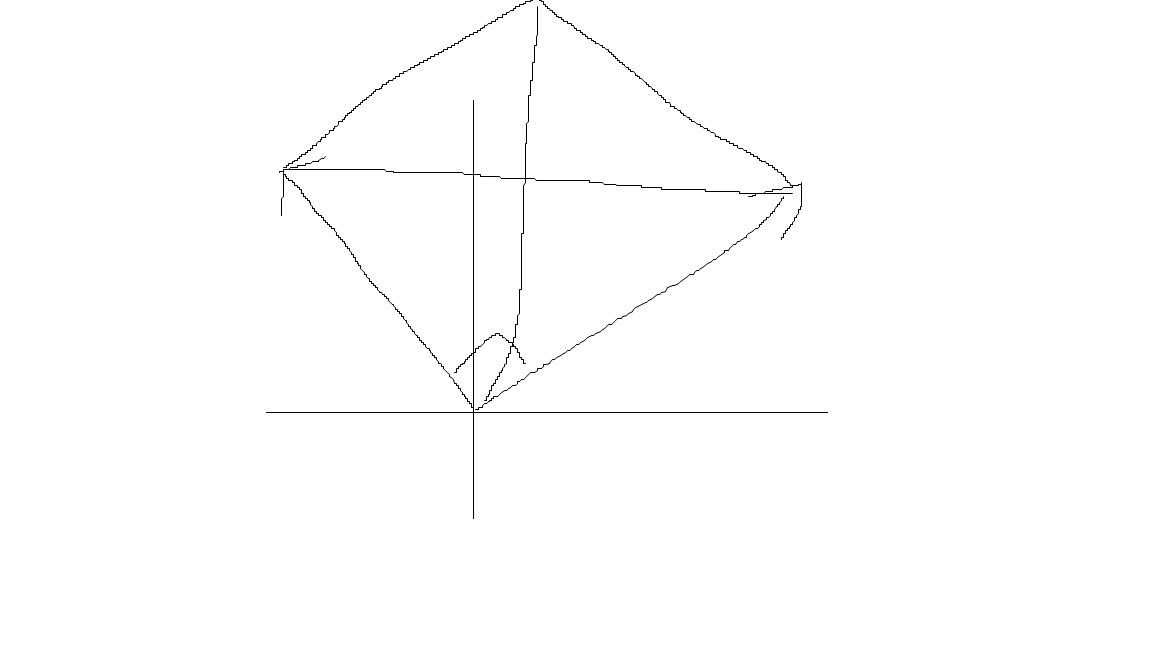
\includegraphics[width=0.7\textwidth]{images/math/1.jpg} %插入图片,[]中设置图片大小,{}中是图片文件名
    % \caption{Main name 2} %最终文档中希望显示的图片标题
    % \label{Fig.main2} %用于文内引用的标签
  \end{figure}
  由于两个向量组成了直角三角形,由勾股定理可知斜边长的平方
  为$v_1^2+v_2^2+w_1^2+w_2^2$. 由于矩形的两个对角线相等,所以该斜边长等于另一个对角
  线的长度. 另一个对角线的终点坐标
  为$(v_1+w_1,v_2+w_2)$,所以$v_1^2+v_2^2+w_1^2+w_2^2=(v_1+w_1)^2+(v_2+w_2)^2$,化简
  即可得$v_1w_1+v_2w_2=0$. $v_1$	
\end{proof}

\end{document}
